\chapter{Metodologi}
\section{Metode Penelitian}
Penelitian ini dikerjakan dengan metode studi analitik dengan cara mengkaji
metode dan teori yang sudah ada sebelumnya. Perhitungan secara analitis juga dilakukan untuk memperkuat serta membuktikan klaim yang dibuat pada tulisan ini.

\section{Diagram Alir}
Untuk lebih jelasnya, berikut adalah diagram alir untuk proses analisis yang dilakukan terhadap setiap siklus mesin panas kuantum fraksional yang ditinjau.
\begin{figure}[H]
    \centering
    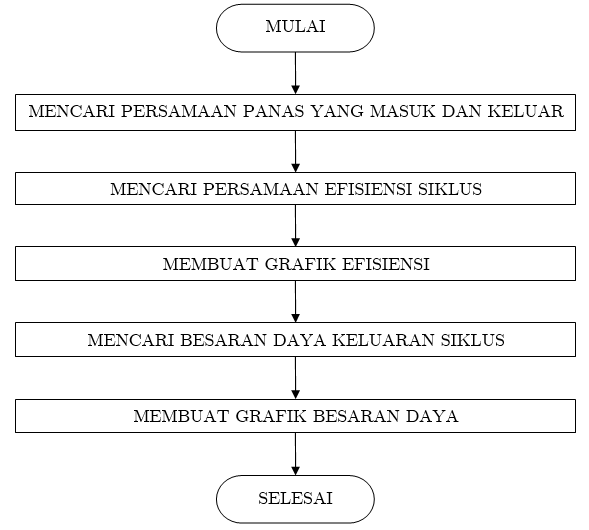
\includegraphics[width=0.7\textwidth]{Images/Diagram Alir.PNG}
    \caption{Diagram alir proses analisis untuk masing-masing siklus mesin panas kuantum fraksional yang ditinjau.}
    \label{fig:DiagramAlir}
\end{figure}

\newpage
\thispagestyle{empty}
\vspace*{\fill}
    \begin{center}
	Halaman ini sengaja dikosongkan
    \end{center}
\vspace*{\fill}
\pagebreak